\chapter{Paralleler Musterabgleich mit regulären Ausdrücken}
\label{sec:regex_naiv}

Aufbauend auf Kapitel \ref{sec:equals_naiv} wird im Folgenden eine komplexere Operation in Form eines Matchers für reguläre Ausdrücke im Kontext der in Kapitel \ref{sec:pipelining} beschriebenen Compiled Query Pipelines auf GPUs untersucht.
Diese Operation stellt wieder eine Selektion über eine Spalte von String-Daten dar, bei der alle Tupel in die Ergebnisrelation übernommen werden, welche dem Muster eines vorgegebenen regulären Ausdrucks entsprechen.

Zunächst wird dazu erläutert, warum das Umsetzen einer solchen Operation im Kontext von Datenbanksystemen relevant ist.
Anschließend wird die allgemeine Struktur der Operation dargestellt, gefolgt von der tatsächlichen Umsetzung des Musterabgleichs mithilfe von Automaten.
Schließlich werden noch einige alternative Verfahren vorgestellt, welche unterschiedliche Eigenschaften aufweisen und mit der vorgestellten Umsetzung verglichen werden.

\section{Motivation}

Die Verwendung von regulären Ausdrücken eröffnet in vielen Anwendungsfällen verschiedenste Möglichkeiten, String-Daten effizient zu verarbeiten und die Leistungsfähigkeiten des Datenbanksystems voll auszunutzen.
Reguläre Ausdrücke stellen ein mächtiges Werkzeug dar, welches den meisten Anwendern von Datenbankmanagementsystemen bekannt ist.
Diese sind vor allem relevant, da sie wie in Kapitel \ref{sec:regex_grundlagen} beschrieben das hoch effiziente Auswerten komplexer Muster erlauben.

Da viele Datenbankmanagementsysteme keine volle Unterstützung für reguläre Ausdrücke bieten, muss eine entsprechende Selektion nach dem Ausführen des Anfrageplans durch das DBMS manuell im Anwendungsprogramm durchgeführt werden.
An dieser Stelle entstehen zahlreiche Probleme, da der Optimierer die Selektion nicht an der optimalen Stelle im Anfrageplan platzieren kann, damit frühzeitig Tupel weg fallen, die nicht in das Ergebnis aufgenommen werden.
Es entsteht also schon beim Datenbankserver eine erhöhte Last durch das unnötige Verarbeiten von Tupeln.
Diese werden zusätzlich noch über das Netzwerk zur Anwendung übertragen, wodurch erneut eine erhöhte Netzlast entsteht.
Die Anwendung wiederum muss anschließend mit einer potenziell geringeren Leistungsfähigkeit als der Datenbankserver die Selektion durchführen, wodurch an dieser Stelle wieder eine unnötig hohe Last entsteht.
Sollten also Anwendungsfälle auftreten, bei denen eine Selektion durch reguläre Ausdrücke gewünscht ist, stellt die Unterstützung dieser Operation durch das Datenbankmanagementsystem einen massiven Vorteil dar.

\section{Struktur der Operation}

Zunächst wird die vorgestellte Operation ohne tiefgreifende Optimierungen implementiert, um damit eine Basis für das Entwickeln einer Verbesserung zu bieten.
Für das Verarbeiten des regulären Ausdrucks wird ein deterministischer Automat erstellt, der genau dann akzeptiert, wenn der aktuell überprüfte String in das Muster des regulären Ausdrucks passt.

Das allgemeine Vorgehen der Operation ist ähnlich zu dem in Kapitel \ref{sec:equals_umsetzung} beschriebenen einfachen String-Vergleich.
Jedem Thread der GPU wir ein Tupel zugewiesen, welcher mithilfe des Automaten untersucht werden soll.
Nachdem der aktuelle Zustand des DFA auf den Startzustand gesetzt wurde, wird der String Zeichen für Zeichen durchlaufen, wobei der Zustand in jedem Schritt entsprechend der Regeln des Automaten aktualisiert wird.
Sobald die Zeichenkette vollständig durchlaufen wurde, wird geprüft, ob sich der Automat in einem akzeptierenden Zustand befindet, in welchem Fall der gesuchte String in das Muster des regulären Ausdrucks passt.
Ist am Ende kein akzeptierender Zustand erreicht, oder wurde die Untersuchung vorzeitig abgebrochen, weil ein Fehlerzustand erreicht wurde, wird das Tupel nicht in das Ergebnis übernommen.

Bei der Ausführung wird der gesamte Warp parallel abgearbeitet, wodurch die Positionen, an denen die Strings untersucht werden für alle Lanes identisch sind.
Außerdem wird das Ergebnis erst geschrieben, sobald alle Threads ihren String vollständig durchlaufen haben oder einen Fehlerzustand erreicht haben.
Schließlich wird jedem Thread eine neue Zeichenkette zugewiesen, mit der das Verfahren wiederholt wird bis sämtliche Tupel abgearbeitet sind.

\newpage

\begin{lstlisting}[language=MyC++,
caption=Naive Implementierung einer Selektion mit einem regulären Ausdruck,
label=naive_regex]
/* execute previous operators in the pipeline */

char *p = data_content + char_offset[loop_var];
char *pe = data_content + char_offset[loop_var + 1];

int cs = machine_start;

while(active) {
	cs = singleDfaStep(cs, p);
	
	p++;
	
	if (p == pe)		// string completely processed
		active = false;
	
	if (cs == 0)		// invalid state reached
		active = false;
}

active = cs >= machine_first_final;

/* execute following operators in the pipeline */
\end{lstlisting}

In Listing \ref{naive_regex} wird die Implementierung des Operators vorgestellt, der im Kontext der kompilierten Anfragepipelines die Selektion über einen regulären Ausdruck ausführt.
Die Datensätze \texttt{data\_content} und \texttt{char\_offset} enthalten wie in Kapitel \ref{sec:equals_umsetzung} die Zeichenketten aus der zu untersuchenden Spalte und die Indizes der einzelnen Tupel innerhalb des Datensatzes.

Zunächst wird die Lane initialisiert, indem ein Zeiger \texttt{p} auf den Anfang des zu untersuchenden Strings und der Zeiger \texttt{pe} auf das Ende gesetzt wird.
Außerdem wird der aktuelle Zustand \texttt{cs} auf den Startzustand des Automaten gesetzt.

In der Schleife wird anschließend über den gesamten String iteriert und dabei mithilfe der Methode \texttt{singleDfaStep} der Folgezustand des Automaten nach Einlesen des nächsten Zeichens bestimmt.
Daraufhin wird überprüft, ob der iterierende Zeiger \texttt{p} auf das Ende des Strings \texttt{pe} zeigt, in welchem Falle dieser vollständig durchlaufen wurde und die Lane vorerst deaktiviert werden kann.
Die Lane wird ebenfalls deaktiviert, wenn der Fehlerzustand \texttt{0} erreicht wurde, von dem aus ein Erreichen eines akzeptierenden Zustandes unmöglich ist.

Nachdem sämtliche Lanes ihre Berechnung abgeschlossen haben, wird überprüft, ob der aktuelle Zustand des DFA zu der Gruppe der akzeptierenden Zustände gehört.
Ist dies der Fall wird die Lane für folgende Operationen aktiviert, ansonsten bleibt diese deaktiviert, sodass die Folgeoperationen nicht ausgeführt werden müssen.

\section{Erstellen und Durchlaufen des Automaten}

Das vorgestellte Verfahren generiert vor der Ausführung des Anfrageplans einen deterministischen Automaten, welcher beim kompilieren der Anfragepipeline in den Kernel eingebaut wird.
Der Automat wird mithilfe des Ragel State Machine Compilers \cite{Thurston2009} erzeugt, auf dem auch der Code zur Verarbeitung des Automaten basiert.

Ragel ermöglicht es, für das Auswerten eines gegebenen regulären Ausdrucks C-Code zu erzeugen, der automatisch in ein vorgegebenes Rahmenprogramm eingefügt wird.
Somit ist es leicht möglich, den Automaten in den Rahmen einer kompilierten Anfragepipeline einzupflegen, es müssen also keinerlei Schnittstellen zu anderen Sprachen oder Konzepten erstellt werden.

Der generierte Code lässt sich in zwei Hauptbestandteile aufteilen.
Zum einen wird etwas Code zur tatsächlichen Durchführung des Musterabgleichs generiert, welcher für unterschiedliche Ausdrücke größtenteils identisch ist.
Außerdem werden einige Tabellen generiert, welche die tatsächlichen Zustände und Zustandsübergänge des Automaten beinhalten und für jeden regulären Ausdruck neu generiert werden müssen.

 \begin{lstlisting}[language=MyC++,
 caption=Methode zur Durchführung eines DFA-Schrittes,
 label=naive_regex_singledfastep]
 __device__ int singleDfaStep(int cs, char* p) {
	 int _slen;
	 int _trans;
	 const char *_keys;
	 const char *_inds;
	 
	 _keys = _machine_trans_keys + (cs<<1);
	 _inds = _machine_indicies + _machine_index_offsets[cs];
	 
	 _slen = _machine_key_spans[cs];
	 _trans = _inds[ _slen > 0 && _keys[0] <=(*p) &&
		 (*p) <= _keys[1] ?
		 (*p) - _keys[0] : _slen ];
	 
	 return _machine_trans_targs[_trans];
 }
 \end{lstlisting}
 
 Listing \ref{naive_regex_singledfastep} zeigt die Methode zur Durchführung eines DFA-Schrittes, welche in Listing \ref{naive_regex} verwendet wird.
 Die Implementierung basiert auf dem durch Ragel erzeugten Ausführungscode, welcher mit der \emph{flat}-Einstellung generiert wurde.
 Dies stellt den simpelsten Code dar, der von Ragel generiert wird, welcher sehr ähnlich zu dem in Kapitel \ref{sec:regex} vorgestellten Prinzip ist.
 Hier werden die ebenfalls von Ragel generierten und in Listing \ref{naive_regex_felder} dargestellten Felder verwendet, welche den eigentlichen DFA enthalten.
 In diesem Beispiel handelt es sich um den Automaten, der aus dem Ausdruck \texttt{(0|1)*((00)+|001)0} generiert wurde.
 
 \newpage
 
 \begin{lstlisting}[language=MyC++,
 caption=Methode zur Durchführung eines DFA-Schrittes,
 label=naive_regex_felder]
static const char _machine_trans_keys[] = {
	0, 0, 0, 1, 0, 1, 0, 1, 0, 1, 0, 1, 0, 1, 0
};

static const char _machine_key_spans[] = {
	0, 2, 2, 2, 2, 2, 2
};

static const char _machine_index_offsets[] = {
	0, 0, 3, 6, 9, 12, 15
};

static const char _machine_indicies[] = {
	0, 2, 1, 3, 2, 1, 4, 
	5, 1, 6, 2, 1, 4, 5, 1, 
	3, 2, 1, 0
};

static const char _machine_trans_targs[] = {
	2, 0, 1, 3, 5, 4, 6
};

static const int machine_start = 1;
static const int machine_first_final = 5;
\end{lstlisting}
 
Da diese Darstellung des Automaten für den Menschen kaum lesbar ist und ein Debugging somit sehr aufwändig werden würde, bietet Ragel außerdem ein Werkzeug zur Visualisierung des Graphen.
Abbildung \ref{ragel_visualisierung} zeigt dazu die visuelle Darstellung des erzeugten DFA.

\begin{figure}[ht]
	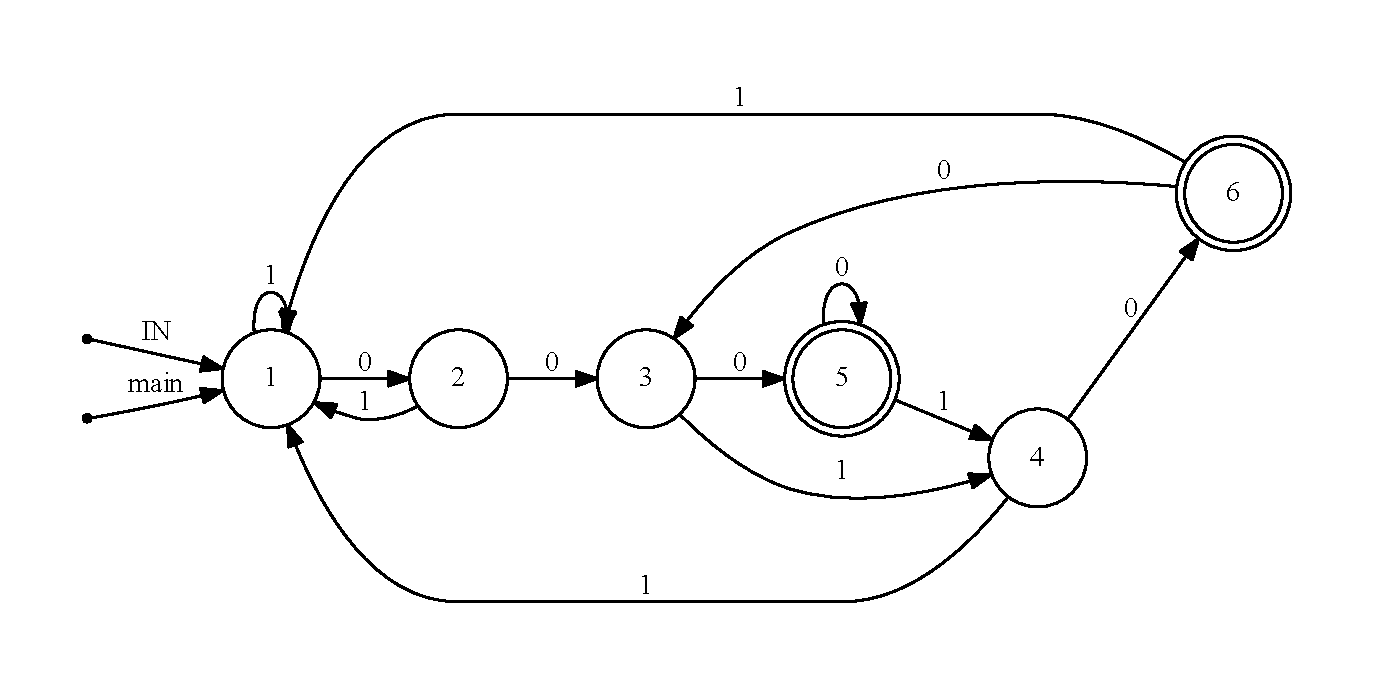
\includegraphics[width=\textwidth]{bilder/ragel_visualisierung.pdf}
	\caption{Visuelle Darstellung des DFAs zum regulären Ausdruck \texttt{(0|1)*((00)+|001)0}}
	\label{ragel_visualisierung}
\end{figure}

\section{Alternative Verfahren}

Zusätzlich zur \emph{flat}-Einstellung, erlaubt Ragel außerdem eine Generierung von Code, welche für die Verarbeitung regulärer Ausdrücke mit einem großen Alphabet optimiert wurde.
Diese Option kann über die \emph{table}-Einstellung abgerufen werden.
Im Gegensatz zur \emph{flat}-Einstellung wird das aktuell untersuchte Zeichen nicht als Index für einen Array von Zustandsübergängen verwendet, sondern in diesem Array eine binäre Suche nach der korrekten Transition durchgeführt.
Nach Thurston ist die oben beschriebene \emph{flat}-Option generell schneller, sie lässt sich allerdings nur für ein kleines Alphabet anwenden \cite{Thurston2009}.
Da im Datenbankkontext generell eher simplere Ausdrücke zu erwarten sind, ist es für die meisten Anwendungsfälle zwar ausreichend, die einfache und schnelle Implementierung zu wählen, es wäre aber auch interessant zu untersuchen, wie groß der Leistungsverlust mit der alternativen Implementierung aussieht, falls komplexere Ausdrücke untersucht werden sollen.

Als Alternative zur vollumfänglichen Unterstützung von regulären Ausdrücken bieten viele Datenbankmanagementsysteme den \emph{LIKE}-Operator an, welcher den einfachen String-Vergleich um Platzhalter erweitert.
So ist es dem Nutzer möglich anstelle des genauen Suchstrings ein Muster anzugeben, in dem Platzhalter für beliebige Zeichen enthalten sind.
Mithilfe dieser simpel umzusetzenden Operation lassen sich viele einfache Abfragen an eine Datenbank modellieren, sodass in vielen Fällen kein richtiger regulärer Ausdruck benötigt wird.
Es wäre daher interessant zu sehen, wie sich die Leistungsfähigkeit dieser Operation mit geringerem Funktionsumfang gegenüber der Umsetzung eines vollständigen Matchers für reguläre Ausdrücke verhält.